\documentclass{elegantbook}

\author{Miao}
\date{\today}
\email{chenmiao.ku@gmail.com}
\usepackage{ntheorem}
\zhtitle{基于计算机网络笔记}
\entitle{Computer Network Note}
\enend{笔记}
\version{0.10}
\myquote{Victory won\rq t come to us unless we go to it.}
\logo{ElegantLaTeX_green.pdf}
\cover{cover.pdf}

\usepackage{listings}
\usepackage{xcolor}
\usepackage{makecell}
\usepackage{lipsum}
\usepackage{texnames}
\usepackage{multirow}

\lstset{ 
  backgroundcolor=\color{white},   % 选择代码背景,必须加上\ usepackage {color}或\ usepackage {xcolor}.
  basicstyle=\bf,                  % 设置代码字号.
  breakatwhitespace=false,         % 设置是否当且仅当在空白处自动中断.
  breaklines=true,                 % 设置自动断行.
  captionpos=b,                    % 设置标题位置.
  commentstyle=\color{red},        % 设置注释格式
  deletekeywords={...},            % 是否删除给定语言的关键词.
  escapeinside={\%*}{*)},          % 是否在代码中添加LaTex.
  extendedchars=true,              % 是否允许使用非ASCII字符; 仅适用于8位编码,不适用于UTF-8. 
  frame=single,	                   % 给代码区添加边框.
  keepspaces=true,                 % 保留空格(useful for keeping indentation of code (possibly needs columns=flexible).
  keywordstyle=\color{blue},       % 关键字显示风格.
  language=C++,                    % 使用的语言.
  morekeywords={*,...},            % 是否需要添加其他的关键词.
  numbers=left,                    % 给代码添加行号,可取值none, left, right.
  numbersep=5pt,                   % 设置行号与代码之间的间隔
  numberstyle=\bf\color{blue},     % 行号的字号和颜色
  rulecolor=\color{black},         % 边框颜色,如果没有设置,框架颜色可以在非黑色文本中的换行符上更改(例如 text (e.g. comments (green here)))
  showspaces=false,                % 显示每个地方添加特定下划线的空格; 覆盖了'showtringspaces'
  showstringspaces=false,          % 仅在字符串中允许空格
  showtabs=false,                  % show tabs within strings adding particular underscores
  stepnumber=2,                    % the step between two line-numbers. If it's 1, each line will be numbered
  stringstyle=\color{green},       % string literal style
  tabsize=4,	                     % 将默认tab设置为2个空格
  title=\lstname                   % show the filename of files included with \lstinputlisting; also try caption instead of title
}


\begin{document}
    \maketitle
    \tableofcontents
    \chapter{绪论}

\section{操作系统基本概念}

    \emph{任何计算机系统都包含一个名为操作系统的基本程序集合。}在这个集合中,最重要的程序称为内核(kernel)。启动后,内核中包含了系统运行所必不可少的很多核心过程(procedure),和其他一些不太重要的实用程序。

    \emph{系统根本的样子和能力还是由内核决定,内核也为操作系统中所有事情提供了主要功能,并决定高层软件的很多特性。}

    操作系统必须完成两个主要目标:

\begin{itemize}
    \item [1)] 与硬件部分交互,为包含在硬件平台上的所有底层可编程部件提供服务
    \item [2)] 为运行在计算机系统上的应用程序提供执行环境
\end{itemize}

    \emph{类Unix系统把与计算机物理组织相关的所有底层细节都对用户运行的程序隐藏起来,硬件为CPU引入了至少两种不同的执行模式:非特权模式(用户态(User Mode)和特权模式(Kernel Mode))}。

\section{多用户系统}

    \emph{多用户系统(multiuser system)就是一台能并发和独立地执行分别属于两个或多个用户的若干应用程序的计算机。}

    并发(concurrently)意味着几个应用程序能够同时处于活动状态并竞争各种资源。独立(independently)意味着每个应用程序能够执行自己的任务,而无需考虑其他用户的应用程序在做什么。

    多用户操作系统必须包含:

\begin{itemize}
    \item [1)] 核实用户身份的认证机制
    \item [2)] 防止有错误的用户程序妨碍其他应用程序在系统中运行的保护机制
    \item [3)] 防止有恶意的用户程序干涩或窥视其他用户的活动的保护机制
    \item [4)] 限制分配给每个用户的资源数的记账机制
\end{itemize}

\section{用户和组}

    操作系统必须保证用户空间的私有部分仅仅对于其拥有者是可见的。

    所有的用户由一个唯一的数字来表示,这个数字叫用户标识符(User ID, UID)。

    为了和其他用户有选择地共享资料,每个用户是一个或多个用户组的一名成员,组由唯一的用户组标识符(user group ID)标识。每个文件也恰好与一个组相对应。

    \emph{任何类Unix操作系统都有一个特殊的用户,root(超级用户(superuser))}。系统管理员能够通过root账号登陆,值得一提的是:\emph{root几乎无所不能,其能访问系统中的每一个文件,能干涉每一个正在执行的用户程序}。

\section{进程}

    \emph{所有的操作系统都有一种基本的抽象:进程(process)。一个进程可以定义为:"程序运行时的一个实例",或者一个运行程序的"执行上下文"}。

    传统的操作系统中,\emph{一个进程在地址空间中(address space)执行一个单独的指令序列。}现代操作系统允许具有多个执行流的进程,也就是在相同的地址空间可执行多个指令序列。

    \emph{允许进程并发活动的系统称为多道程序系统(multiprogramming)或多处理系统(multiprocessing)}。值得注意的是:几个进程能够并发地执行同一个程序,而同一个进程能顺序的执行几个程序。

    调度程序(scheduler)的部分决定哪个进程能执行,一些操作系统只允许有非抢占式(nonpreemptable)进程,\emph{也就是说,只有当进程自愿放弃时,调度程序才能被调用。但是,多用户系统中的进程必须是抢占式的(preemptable)}。

\section{内核体系结构}

    大部分Unix内核都是单块结构:\emph{每一个内核层都被集成到整个内核程序中,并代表当前进程在内核态下运行。}

    \emph{微内核(microkernel)操作系统只需要内核有一个很小的函数集(几个同步原语\footnote[1]{原语(primitive)是计算机科学中的一个概念,它指的是一组基本的操作或指令,可以直接在计算机硬件上执行。原语通常是由计算机硬件提供的,用于支持高级编程语言或操作系统的功能},一个简单的调度程序和进程间通信)}。

    Linux内核提供了模块(module)用于达到微内核理论上的很多优点且不影响性能。\emph{模块是一个目标文件,其代码可以在运行时链接到内核或从内核解除链接。这种目标代码通常由一组函数组成,用来实现文件系统、驱动程序或其他内核上层功能。}

    使用模块的主要优点:

\begin{itemize}
    \item [1)] 模块化方法
    \subitem 任何模块都能在运行时被链接或解除链接。这要求程序员提出良定义的软件接口以访问由模块处理的数据结构
    \item [2)] 平台无关性
    \subitem 即使模块依赖于某些特殊的硬件特点,但它不依赖于某个固定的硬件平台
    \item [3)] 节省内存使用
    \subitem 当需要模块时,就链接;不需要时,则解除
    \item [4)] 无性能损失
    \subitem 模块的目标代码一旦被链接进内核,起作用与静态链接的内核的目标代码完全对等。因此无需显式的进行消息传递\footnote[1]{模块被链接或解除时,都有一定的性能下降。但是在微内核中也是如此}
\end{itemize}

\section{Unix文件系统概述}

\subsection{文件}

    \emph{Unix文件是以字节序列组成的信息载体(container),内核不解释文件的内容。}

    从用户的观点来看,文件被组织在一个树结构的命名空间内:

\begin{figure}[!htbp]
    \centering
    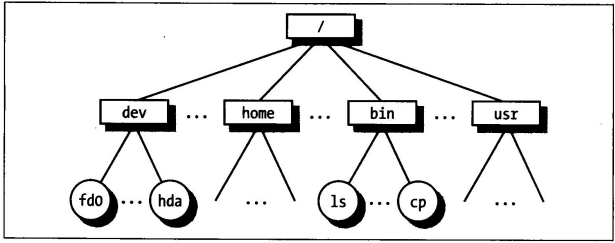
\includegraphics[width=0.6\textwidth]{image/chapter01/目录树结构.png}
    \caption{目录树结构}
\end{figure}

    除叶节点外,所有节点都表示目录名。目录节点包含它下面文件及目录的所有信息。

    \emph{Unix每个进程都有一个当前工作目录,属于进程执行上下文(execution context),标识出进程所用的当前目录。}

    \emph{路径名(pathname)由斜杠及一列指向文件的目录名交替组成。如果第一个字符是斜杠,那么就是所谓的绝对路径;否则就是所谓的相对路径。}

    当标识文件名时,用符号"."和".."分别标识当前工作目录和父目录。

\subsection{硬链接和软连接}

    \emph{包含在目录中的文件名就是一个文件的硬链接(hard link),或简称连接(link)。}

    使用Unix命令:

\begin{lstlisting}[language=C++]
$ ln P1 P2
\end{lstlisting}

    用来创建一个新的硬链接,即为由路径P1标识的文件创建一个路径名为P2的硬链接。

    硬链接有两方面的限制:

\begin{itemize}
    \item [1)] 不允许给目录创建硬链接,这可能使得目录树编程环形图从而无法通过名字定位一个文件
    \item [2)] 只有在同一文件系统中的文件之间才能创建链接。
\end{itemize}

    为了克服限制,引入\emph{软链接(soft link)[也称符号链接(symbolic link)],符号链接是短文件,这些文件包含另一个文件的任意一个路径名。}

    值得注意的是:\emph{路径名可以指向位于任意一个文件系统的任意文件或目录(哪怕它不存在)}。

    Unix命令:

\begin{lstlisting}[language=C++]
$ ln -s P1 P2
\end{lstlisting}

    创建一个路径名为P2的新软连接,P2指向路径名P1。当执行命令时,文件系统抽取P2的目录部分,并在此创建P2的符号链接属性的新项。因此,任何对P2的引用都可以自动被转换为指向P1的引用。

\subsection{文件类型}

    Unix命令文件可以是以下类型:

\begin{itemize}
    \item 普通文件(regular file)
    \item 目录
    \item 符号链接
    \item 面向块的设备文件(block-oriented device file)
    \item 面向字符的设备文件(character-oriented device file)
    \item 管道(pipe)和命名管道(named pipe)(也叫FIFO)
    \item 套接字(socket)
\end{itemize}

\subsection{文件描述符与索引节点}

    \emph{除了设备文件和特殊文件系统外,每个文件都由字符序列组成。文件内容不包括任何控制信息,如文件长度或文件结束符(end-of-file, EOF)}。

    \emph{文件系统处理文件需要的所有信息都包含在一个名为索引节点(inode)的数据结构中,文件系统用索引节点来标识文件。}

    索引节点(inode)至少包括:

\begin{itemize}
    \item 文件类型
    \item 与文件相关的硬链接个数
    \item 以字节为单位的文件长度
    \item 设备标识符(即包含文件的设备的标识符)
    \item 文件系统中标识的索引节点号
    \item 文件拥有者的UID
    \item 文件的用户组ID
    \item 几个时间戳(改变时间、最后访问时间、最后修改时间)
    \item 访问权限和文件模式
\end{itemize}

\subsection{访问权限和文件模式}

    文件的潜在用户分为三种类型:

\begin{itemize}
    \item 文件所有者
    \item 同组用户(不含所有者)
    \item 其他用户
\end{itemize}

    同时,拥有三种类型的访问权限————读、写以及执行。因此就有九种组合不同的二进制来标记,还有三种额外的标记

\begin{itemize}
    \item suid
    \subitem 进程执行一个文件时通常保持进程拥有者的UID,若设置suid,进程就可以获取该文件拥有者的UID
    \item sgid 
    \subitem 进程执行一个文件时保持进程组的用户组ID,若设置sgid,进程就可以获得该文件用户组ID
    \item sticky
    \subitem 设置sticky标志位相当于向内核发出请求,当程序结束后仍保留在内存\footnote[1]{该标记已经过时,已被其他方法取代}
\end{itemize}


    \chapter{进程与线程}

\section{进程与线程}

\subsection{进程的概念和特征}

    通常而言,在不同的认知角度上,对进程的定义是不同的,比较典型的定义为:

\begin{itemize}
    \item [1)] 进程是程序的一次执行过程
    \item [2)] 进程是一个程序及其数据在处理及上顺序执行时所发生的活动
    \item [3)] 进程是具有独立功能的程序在一个数据集合上运行的过程,是系统进行资源分配和调度的一个独立单位。
\end{itemize}

    当然的,在OS中,进程经过了抽象从而定义了一个重要的数据结构:进程控制块(Process Control Block,PCB)\footnote[1]{\emph{Linux中为task\_struct,定义在sche.h文件中}}。系统利用PCB来描述进程的基本情况和运行状态,进而控制和管理进程。\emph{相应地,由程序段、相关数据段和PCB三部分构成了进程实体(进程映像)。}

    注意:\emph{\color{red}PCB是进程存在的唯一标识}。

    \emph{进程映像可以被视为进程在内存中的静态表示,描述了进程的初始状态和资源分配情况。虽然进程映像在进程运行期间保持不变,但进程本身可能会发生动态的变化。}

    注意:\emph{\color{red}进程映像是静态的,进程则是动态的。}

    引入进程映像的概念后,又有了新的定义:\emph{进程是进程映像的运行过程,是系统进行资源分配和调度的一个独立单位。}

    进程是由多道程序的并发执行而引出的,其基本特征是对比单个程序的顺序执行提出的,也是对进程管理的基本要求:

\begin{itemize}
    \item [1)] 动态性。进程是程序的一次执行,{\color{red}动态性是进程最基本的特征}。
    \item [2)] 并发性。多个进程映像同存于内存中,能在一段时间内同时运行。{\color{red}并发性是进程的重要特征,也是OS的重要特征}。
    \item [3)] 独立性。进程映像是一个能独立运行、独立获得资源和独立接受调度的基本单位(此处暂时不考虑线程)。
    \item [4)] 异步性。由于进程的互相制约,使得进程各自独立、不可预知的向前推进。\emph{\color{red}异步性会导致执行的不可再现性,因此必须配置同步机制}。
\end{itemize}

\subsection{进程的状态与转换}

    进程在其生命周期内,会不断地发生状态变化。通常进程有五种状态,前三种是基本状态:

\begin{itemize}
    \item [1)] 运行态(Running)。进程正在CPU上运行。
    \item [2)] 就绪态(Runable)。进程获得了除处理机外的一切所需资源,\emph{通常处于就绪态的进程有多个,因此OS用就绪队列组织。}
    \item [3)] 阻塞态(Blocking/Waiting)。进程正在\emph{等待某一事件而暂停,通常处于阻塞态的进程有多个,因此OS用阻塞(等待)队列来组织,甚至可以根据阻塞原因设置多个阻塞队列。}
    \item [4)] 创建态(Creating)。进程正在被创建,未转到就绪态。
    \item [5)] 终止态(Exiting)。进程正在被释放或结束。
\end{itemize}

\begin{figure}[!htbp]
    \centering
    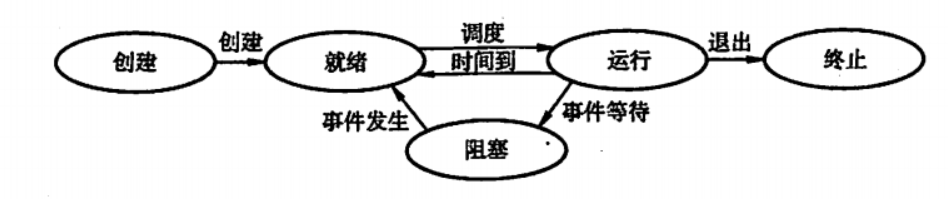
\includegraphics[width=0.8\textwidth]{image/chapter02/五种状态的转换.png}
    \caption{五种状态的转换}
\end{figure}

    值得注意的是:\emph{就绪态是指仅仅缺少处理机资源,也就是在就绪队列中还未到其处理的事件。而阻塞态是指,既缺乏处理机资源,又缺乏运行所需的必要资源(或事件发生)。}

    \emph{\color{red}一个进程从运行态变为阻塞态是主动的行为,从阻塞态变成就绪态是被动的行为。同时,就绪态不可能直接变为阻塞状态,因为变成阻塞必定是申请某种资源或事件发生,而这种情况之可能发生在运行时。}

\subsection{进程的组成}

    进程是一个独立的运行单位,也是OS进行资源分配和调度的基本单位。其由三个部分组成

\subsubsection{进程控制块}

    进程创建时,需要新建一个PCB常驻于内存中,PCB是进程存在的唯一标识,也是进程映射的一部分。

    \emph{在整个生命周期中,系统总是通过PCB对进程进行控制的,即系统唯有通过进程的PCB才能感知到该进程的存在。}

\begin{table*}[!htbp]
    \begin{center}
        \caption{PCB通常包含的内容}
        \begin{tabular}{c | c | c | c}
            \hline
            进程描述信息 & 进程控制和管理信息 & 资源分配清单 & 处理机相关信息 \\
            \hline
            进程标识符(PID) & 进程当前状态 & 代码段指针 & 通用寄存器值 \\
            \hline
            用户标识符(UID) & 进程优先级 & 数据段指针 & 地址寄存器值 \\
            \hline
            & 代码运行入口地址 & 堆栈指针 & 控制寄存器值 \\
            \hline
            & 程序外存地址 & 文件描述符 & 标志寄存器值 \\
            \hline
            & 进入内存时间 & 键盘 & 状态字 \\
            \hline
            & 处理机占用时间 & 鼠标 & \\
            \hline
            & 信号量使用 & & \\
            \hline
        \end{tabular}
    \end{center}
\end{table*}

\begin{itemize}
    \item [1)] 进程描述信息。\emph{\color{red}PID是进程的唯一标识符}。UID标识了进程所属的用户
    \item [2)] 进程控制和管理信息。
    \subitem 进程当前状态:描述进程的状态信息,作为调度的凭据
    \subitem 进程优先级:用于抢占机制
    \item [3)] 资源分配清单。用于说明内存地址空间或虚拟地址空间的状态,以及文件和I/O情况
    \item [4)] 处理机相关信息。用于保存进程的信息,当进程被切换时,必须将上下文信息保存在此处(线程就是为此的)。
\end{itemize}

    在OS中,为了满足各种情况,通常有:就绪队列,等待队列以及优先级队列,这三种队列都会保存在PCB中以供使用。

    特别的,一般而言还有另外一种组织方式:索引方式,将同一状态的进程组织在一张索引表内,然后通过索引表项指向PCB。

\subsubsection{程序段}

    程序段就是\emph{能够被进程调度程序调度到CPU执行的程序段代码。程序可能被多个进程共享。}

    代码段通常是只读的,意味着程序在运行时无法修改代码段中的指令。这是为了确保程序的逻辑和一致性。如果程序需要修改自身的指令,通常会使用特殊的技术,如自修改代码或动态代码生成。

    在计算机的内存中,代码段通常位于程序的虚拟地址空间的一个固定位置。操作系统负责将代码段加载到内存中,并为程序提供执行的环境和资源。

\subsubsection{数据段}

    一个进程的数据段,\emph{可以是进程对应的程序加工处理的原始数据,也可以是程序执行时产生的中间或最终结果。}

    进程的可变性,就主要体现在数据段中的变化。

\subsection{进程控制}

    进程控制的主要功能是对系统中的所有进程实施有效的控制,具有创建、删除、转换等原语。

\subsubsection{进程的创建}

    允许一个进程创建另一个进程。子进程可以继承父进程的所有资源。在OS中,系统调用的上层接口是fork(),而底层的原语接口是clone()。

    在OS中,终端用户登录系统、作业调度、系统提供服务、用户程序的应用请求等都会引起进程的创建:

\begin{itemize}
    \item [1)] 为新进程分配唯一的一个PID,并申请一个空白PCB。
    \item [2)] 为进程分配运行所需的各种资源。
    \item [3)] 初始化PCB,主要包括初始化标志信息、初始化CPU状态信息和初始化CPU控制信息,以及设置优先级
    \item [4)] 若进程就绪队列能够容纳,则并入就绪队列,等待被调度
\end{itemize}

\subsubsection{进程的终止}

    引起进程终止的事件主要有:正常结束;异常结束;外界干预这三种:

\begin{itemize}
    \item [1)] 根据被终止进程的标识符,检索出进程的PCB,从中读取进程状态
    \item [2)] 若被终止进程处于运行态,立即终止执行,并将处理机资源分配给其他任务
    \item [3)] 若该进程有子进程,则还应将子进程终止
    \item [4)] 将该进程的全部资源归还给父进程或OS
    \item [5)] 将该PCB从队列中移除
\end{itemize}

\subsubsection{进程的阻塞和唤醒}

    正在运行的任务,由于期待的事件尚未发生,进程便通过调用阻塞原语,使自身从运行态转变为阻塞状态。\emph{可见,阻塞态是一种进程的自身主动行为,因此只能处于在运行态的进程才可能转换为阻塞态}:

\begin{itemize}
    \item [1)] 找到将要被阻塞进程的标识号对应的PCB
    \item [2)] 若进程为运行态,则{\color{red}保护现场},将其转换为阻塞态,停止运行
    \item [3)] 将该PCB插入到对应事件的等待队列,将处理机资源调度给其他就绪任务
\end{itemize}

    当被阻塞进程所期待的事件发生时,由有关进程调用唤醒原语(Wakeup):

\begin{itemize}
    \item [1)] 在该事件的等待队列中找到响应的PCB
    \item [2)] 将其从等待队列中移除,并置为就绪态
    \item [3)] 把该PCB插入就绪队列,等待调度程序调度
\end{itemize}

    注意:\emph{阻塞和唤醒原语是一对作用相反的原语,因此需要成对使用。}

\subsubsection{进程的切换}

    进程的切换一般由于:当前进程时间片到;更高优先级任务到达;当前进程主动阻塞;当前进程终止等,这时就需要切换原语:

\begin{itemize}
    \item [1)] 将运行环境信息存入PCB
    \item [2)] PCB移入对应队列
    \item [3)] 选择另一个任务执行,更新PCB
    \item [4)] 根据PCB恢复新进程所需要的环境
\end{itemize}

    对于切换的原语,可以在内核中轻易的找到:

\begin{lstlisting}[language=C++]
#define switch_to(prev,next,last) \
asm volatile(SAVE_CONTEXT						    \
    "movq %%rsp,%P[threadrsp](%[prev])\n\t" /* save RSP */	  \
    "movq %P[threadrsp](%[next]),%%rsp\n\t" /* restore RSP */	  \
    "call __switch_to\n\t"					  \
    ".globl thread_return\n"					\
    "thread_return:\n\t"					    \
    "movq %%gs:%P[pda_pcurrent],%%rsi\n\t"			  \
    "movq %P[thread_info](%%rsi),%%r8\n\t"			  \
    "btr  %[tif_fork],%P[ti_flags](%%r8)\n\t"			  \
    "movq %%rax,%%rdi\n\t" 					  \
    "jc   ret_from_fork\n\t"					  \
    RESTORE_CONTEXT						    \
    : "=a" (last)					  	  \
    : [next] "S" (next), [prev] "D" (prev),			  \
    [threadrsp] "i" (offsetof(struct task_struct, thread.rsp)), \
    [ti_flags] "i" (offsetof(struct thread_info, flags)),\
    [tif_fork] "i" (TIF_FORK),			  \
    [thread_info] "i" (offsetof(struct task_struct, thread_info)), \
    [pda_pcurrent] "i" (offsetof(struct x8664_pda, pcurrent))   \
    : "memory", "cc" __EXTRA_CLOBBER)

struct task_struct *
__switch_to(struct task_struct *prev_p, struct task_struct *next_p)
\end{lstlisting}

\subsection{进程的通信}

    进程通信是指进程间的信息交换。PV操作是低级通信方式\footnote[1]{\emph{PV操作是一种用于进程同步的经典算法,用于解决进程之间的互斥和同步问题。PV操作通常与信号量(Semaphore)相关联。当进程需要访问共享资源时,执行P(wait)操作;当进程结束访问时,需要执行V(signal)操作。}},高级通信方式是指\emph{以较高的效率传输大量数据的通信方式}。

\subsubsection{共享存储}

    \emph{进程空间一般都是独立的,进程运行期间不能访问其他进程。}这是共享存储的前提条件,在通信的进程之间存在一块可以直接访问的共享空间,通过对该空间进行读写操作,实现进程间的消息互换。

\begin{figure}[!htbp]
    \centering
    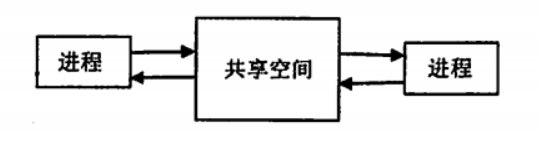
\includegraphics[width=0.6\textwidth]{image/chapter02/共享空间.png}
    \caption{共享存储}
\end{figure}

    为了实现共享存储,一般OS会提供上层接口以供使用。例如Linux中,提供了shm\_*等操作实现申请、撤销共享空间等操作,然后通过mmap将共享空间映射到进程自身的空间中。

    此处给出简单的示例:

\begin{lstlisting}[language=C++]
#include <stdio.h>
#include <stdlib.h>
#include <sys/mman.h>
#include <sys/stat.h>
#include <fcntl.h>
#include <unistd.h>
#include <sys/types.h>

int main() {
    const char* shm_name = "/my_shared_memory";
    int shm_fd = shm_open(shm_name, O_RDWR | O_CREAT, 0666);
    if (shm_fd == -1) {
        perror("shm_open");
        exit(1);
    }

    off_t size = 4096; // 共享内存的大小
    if (ftruncate(shm_fd, size) == -1) {
        perror("ftruncate");
        exit(1);
    }

    void* addr = mmap(NULL, size, PROT_READ | PROT_WRITE, MAP_SHARED, shm_fd, 0);
    if (addr == MAP_FAILED) {
        perror("mmap");
        exit(1);
    }

    // 现在可以通过addr指针来访问共享内存中的数据

    // 访问完成后,记得使用munmap函数解除映射
    if (munmap(addr, size) == -1) {
        perror("munmap");
        exit(1);
    }

    // 关闭共享内存文件描述符
    if (close(shm_fd) == -1) {
        perror("close");
        exit(1);
    }

    // 删除共享内存对象
    if (shm_unlink(shm_name) == -1) {
        perror("shm_unlink");
        exit(1);
    }

    return 0;
}
\end{lstlisting}

    对于共享存储而言,拥有两种方式:低级的共享是通过语言特性,例如全局的数据结构的共享,但是这样效率低、局限大;高级的共享就是通过这样实现一块存储区,速度快,局限小。

\subsubsection{消息传递}

    在消息传递系统中,进程间的数据交换以格式化的信息为单位。进程通过系统提供的发送/接收原语进行数据交换,\emph{这种方式隐藏了通信实现细节,使通信过程对用户透明,简化了通信程序的设计,是目前最广泛应用的机制。}

\begin{figure}[!htbp]
    \centering
    
\includegraphics[width=0.4\textwidth]{image/chapter02/消息传递.png}
    \caption{消息传递}  
\end{figure}

\begin{itemize}
    \item [1)] 直接通信方式。发送进程直接把消息发送给接收进程,并将其挂在接收进程的消息缓冲队列上,接收进程从中获取消息。
    \item [2)] 间接通信方式。发送进程把消息发送到某个中间实体(类似于电子邮件的机制,是有一个邮件服务器的缓冲区),接收端从中间实体获取消息,该中间实体一般称为信箱。
\end{itemize}

\subsubsection{管道通信}

    \emph{在Linux中,管道是一种使用非常频繁的通信机制,本质上也是一种文件。}管道通信允许两个进程按生产-消费者模型进行通信,数据在管道中是FIFO的。管道的大小也是有规定的,一般为4KB(也就是说,是一个固定的缓冲区)。

    \emph{1. 管道只能采用半双工通信,某段时间内只能单向通信;但可以使用两个管道实现全双工通信。}

    \emph{2. 各进程需要互斥的读写管道。当管道写满时,写进程阻塞;当管道读空时,读进程堵塞。}

    \emph{3. 数据一旦被读取,一般情况下会消失。因此会出现争议:a). 一个管道允许多个写进程,一个读进程\footnote[1]{\emph{如果是答题,按照参考答案上的结果就是这样。如果从理解上来看,这种和后面一种的方式都是正确的。}}。b). 允许多个写进程,多个读进程,系统会让进程各自轮流读取\footnote[2]{\emph{Linux中的策略}}}。

    一个简单的示例,实现进程间互相通信:

\begin{lstlisting}[language=C++]
#include <stdio.h>
#include <stdlib.h>
#include <unistd.h>

int main() {
    int pipe1[2]; // 管道1,用于父进程向子进程发送数据
    int pipe2[2]; // 管道2,用于子进程向父进程发送数据

    if (pipe(pipe1) == -1 || pipe(pipe2) == -1) {
        perror("pipe");
        exit(1);
    }

    pid_t pid = fork();
    if (pid == -1) {
        perror("fork");
        exit(1);
    }

    if (pid == 0) {
        // 子进程
        close(pipe1[1]); // 关闭管道1的写端
        close(pipe2[0]); // 关闭管道2的读端

        char message[100];
        read(pipe1[0], message, sizeof(message)); // 从管道1读取数据
        printf("子进程收到消息:%s\n", message);

        const char* reply = "Hello, 父进程!";
        write(pipe2[1], reply, strlen(reply) + 1); // 向管道2写入数据

        close(pipe1[0]); // 关闭管道1的读端
        close(pipe2[1]); // 关闭管道2的写端
    } else {
        // 父进程
        close(pipe1[0]); // 关闭管道1的读端
        close(pipe2[1]); // 关闭管道2的写端

        const char* message = "Hello, 子进程!";
        write(pipe1[1], message, strlen(message) + 1); // 向管道1写入数据

        char reply[100];
        read(pipe2[0], reply, sizeof(reply)); // 从管道2读取数据
        printf("父进程收到消息:%s\n", reply);

        close(pipe1[1]); // 关闭管道1的写端
        close(pipe2[0]); // 关闭管道2的读端
    }

    return 0;
}
\end{lstlisting}

\subsection{线程和多线程模型}

\subsubsection{线程的基本概念}

    \emph{引入线程的目的是减少程序在并发执行时所付出的时空开销,提高OS的并发性能。}

    线程最为直接的理解就是“轻量级进程”,\emph{是一个基本的CPU执行单元,也是程序执行流的最小单元。}线程是进程的一个实体,\emph{{\color{red}是被OS独立调度和分派的基本单位}(引入线程后,进程就不再是调度的基本单位了),线程不拥有系统资源,但可以与同属进程的其他线程共享所拥有的全部资源。}

    那么,现在重新定义:\emph{进程是只作为除CPU外的系统资源的分配单元,线程作为处理机的分配单元。}

\subsubsection{线程与进程的比较}

\begin{itemize}
    \item [1)] 调度
    \subitem 引入线程后,\emph{线程是独立调度的基本单位},线程切换的代价远小于进程,同时,在同一进程中的不同线程切换,不需要切换进程。
    \item [2)] 并发性
    \subitem 不仅进程能够并发,线程也是能够并发的,准确来说,线程就是为此而生的
    \item [3)] 拥有资源
    \subitem \emph{进程是系统中拥有资源的基本单位,线程不拥有系统资源,但能够访问所属进程的资源(主要表现在,同一进程中的所有线程具有相同的地址空间)}
    \item [4)] 独立性
    \subitem \emph{每个进程都拥有独立的地址空间和资源,除了共享的全局变量;而同一进程的所属线程间,共享进程的地址空间和资源。}
    \item [5)] 系统开销
    \subitem 显然,线程的各种开销明显小于进程
    \item [6)] 支持多处理机系统
\end{itemize}

\subsubsection{线程的状态和转换}

    与进程类似,各线程间因为并发的原因也存在共享资源和相互合作的制约关系:

\begin{figure}[!htbp]
    \centering
    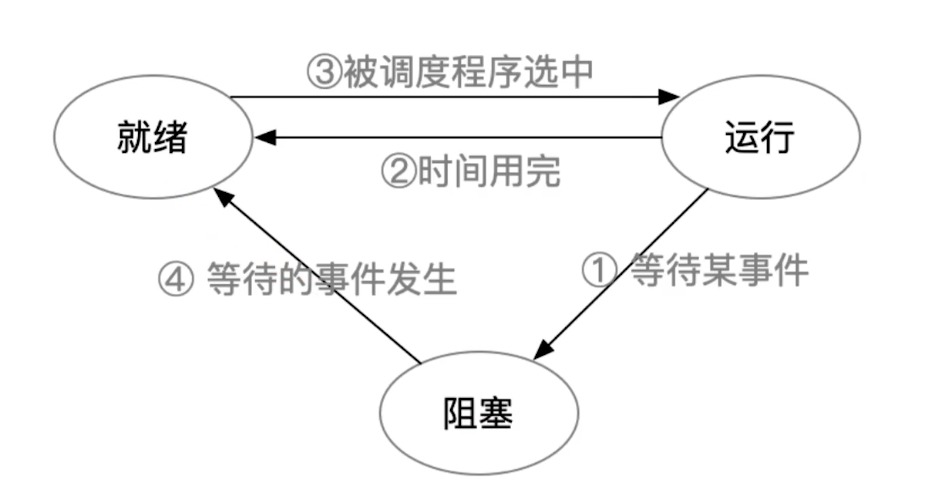
\includegraphics[width=0.6\textwidth]{image/chapter02/线程的状态与转换.png}
    \caption{线程的状态与转换}
\end{figure}

\subsubsection{线程的组织与控制}

    与进程类似,OS也为线程配置了一个线程控制块TCB,用于记录控制和管理线程的信息。

\begin{figure}[!htbp]
    \centering
    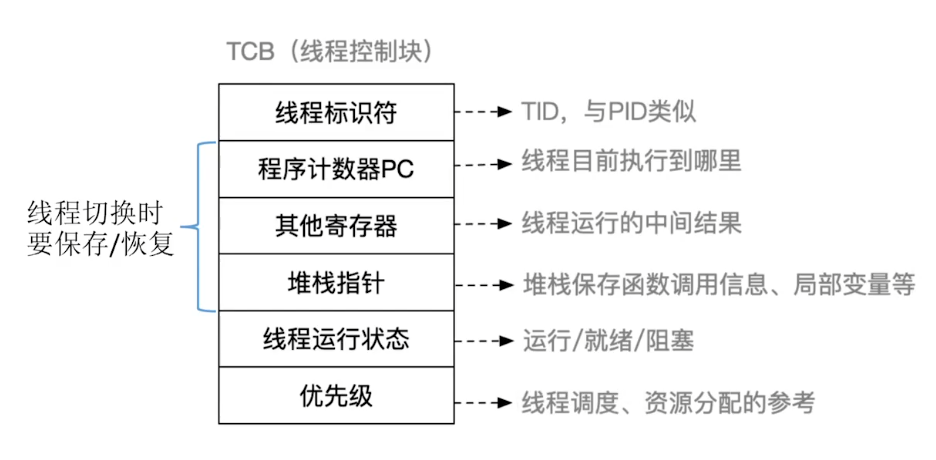
\includegraphics[width=0.6\textwidth]{image/chapter02/TCB.png}
    \caption{TCB}
\end{figure}

    同一进程中所有线程都完全共享进程的空间与资源,一个线程能够读写甚至删除另一个线程的堆栈。同时,线程的创建和终止也和进程类似,不过在删除时,必须考虑进程的因素,从而选择是否释放资源。

\subsubsection{线程的实现方式}

    线程的实现可以分为两类:用户级线程(User-Level Thread,ULT)和内核级线程(Kernel-Level Thread)

\paragraph{用户级线程}

    \emph{在用户级线程中,有关线程管理的所有工作都是由应用程序在用户态完成的,{\color{red}内核根本意识不到线程的存在}。}因此,对于设置了ULT的系统,其调度实际上还是以进程为单位的。

    这种方式的优点在于:

    \emph{1. 线程切换不需要进入到内核态,节省了切换的开销。}

    \emph{2. 调度算法是进程专用的,不同进程可根据自身需求,为自己的线程选择不同的调度算法。}

    \emph{3. 用户级线程的实现与OS无关,对线程管理的代码属于用户程序的一部分}

    而缺点在于:

    \emph{1. 系统调用的阻塞不仅会导致该进程被阻塞,且进程内的所有线程都会被阻塞}

    \emph{2. 严重降低了处理效率,不能发挥多处理机的优势}

\paragraph{内核级线程}

    内核级线程是由内核支持的,线程管理的工作在内核空间中实现。因此内核为每个线程设置了TCB,\emph{\color{red}内核能够对内核级线程进行感知。}

    这种方式的优点在于:

    \emph{1. 发挥了多处理机的优势,能够同时调度同一进程中的多个线程}

    \emph{2. 如果进程中的一个线程阻塞,那么可以对另外一个线程进行调度}

    \emph{3. 内核支持线程具有小的数据结构和堆栈,切换较快,开销较小}

    \emph{4. 内核本身也提供多线程技术,提高系统的执行效率}

    而缺点在于:

    \emph{同一进程中的线程切换,需要转换到内核态,系统开销较大。}

\paragraph{ULT \& KLT}

    ULT和KLT的组合能够使得结合各自的优点并克服各自的不足。支持多个内核级线程的建立、调度和管理,同时允许用户级线程的使用,能够使得线程阻塞但不会导致其他线程阻塞。

\begin{figure}[!htbp]
    \centering
    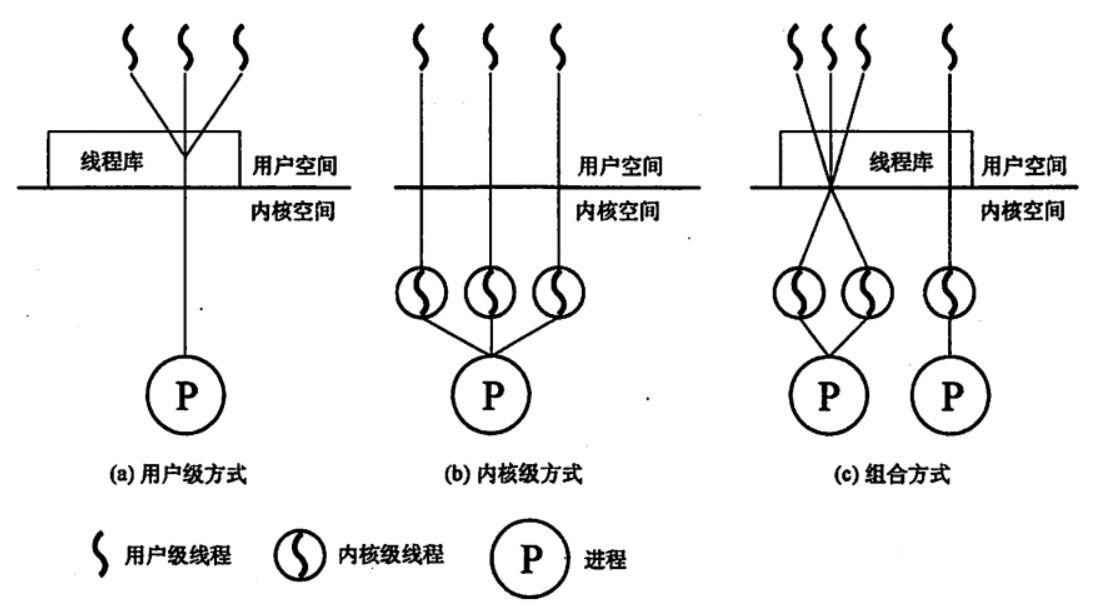
\includegraphics[width=0.8\textwidth]{image/chapter02/用户级线程和内核级线程.png}
    \caption{用户级线程和内核级线程}
\end{figure}

\subsubsection{多线程模型}

    基于有些系统同时支持用户线程和内核线程,因此就会产生不同的多线程模型:

\paragraph{多对一模型}

    将多个用户级线程映射到一个内核级线程(一般来说,多对一就是特指一个内核级线程),这些用户级线程通常属于一个进程。

    优点:线程管理在用户空间进行,效率较高

    缺点:一个线程发生阻塞,那么整个进程都会阻塞;且任何时刻只能由一个线程访问内核

\paragraph{一对一模型}

    每个用户级线程映射到一个内核级线程

    优点:当一个线程被阻塞后,允许调度另一个线程,并发能力较强

    缺点:每创建一个用户线程,都需要一个内核线程,开销过大

\paragraph{多对多模型}

    将n个用户级线程映射到m个内核级线程,要求$n \geq m$

    特点:既克服了多对一模型并发度不高的缺点,又克服了一对一模型开销过大的问题。

\begin{figure}[!htbp]
    \centering
    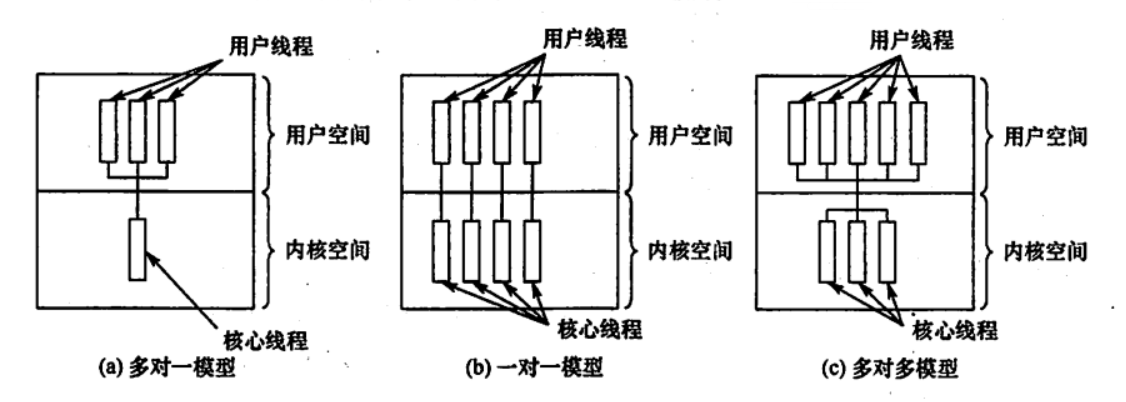
\includegraphics[width=0.8\textwidth]{image/chapter02/多线程模型.png}
    \caption{多线程模型}
\end{figure}


\end{document}
